\documentclass[review]{elsarticle}

\usepackage{lineno,hyperref}
\usepackage{siunitx}
\usepackage{glossaries}
\usepackage{booktabs}
\usepackage[super]{nth}
\usepackage{caption}
\usepackage{mhchem} % Iadded
\usepackage{paralist} %I added

\modulolinenumbers[5]



\journal{Journal of \LaTeX\ Templates}

%%%%%%%%%%%%%%%%%%%%%%%
%% Elsevier bibliography styles
%%%%%%%%%%%%%%%%%%%%%%%
%% To change the style, put a % in front of the second line of the current style and
%% remove the % from the second line of the style you would like to use.Tree View: Show
%%%%%%%%%%%%%%%%%%%%%%%

%% Numbered
%\bibliographystyle{model1-num-names}

%% Numbered without titles
%\bibliographystyle{model1a-num-names}

%% Harvard
%\bibliographystyle{model2-names.bst}\biboptions{authoryear}

%% Vancouver numbered
%\usepackage{numcompress}\bibliographystyle{model3-num-names}

%% Vancouver name/year
%\usepackage{numcompress}\bibliographystyle{model4-names}\biboptions{authoryear}

%% APA style
%\bibliographystyle{model5-names}\biboptions{authoryear}

%% AMA style
%\usepackage{numcompress}\bibliographystyle{model6-num-names}

%% `Elsevier LaTeX' style
\bibliographystyle{elsarticle-num}
%%%%%%%%%%%%%%%%%%%%%%%

%----------------------------------------------------------------------------------------
%	chemins pour les images
%----------------------------------------------------------------------------------------

\graphicspath{{images/}}

\begin{document}

\begin{frontmatter}

\title{Mock--up lime--based paint layer to simulate readhesion interventions}

%% Group authors per affiliation:
\author{Anjo Weichbrodt}

\address{Rue Jean Grimoux 8, 1700 Fribourg}
\ead{anjo.weichbrodt@gmail.com}

%% or include affiliations in footnotes:
%  \author[mymainaddress,mysecondaryaddress]{Elsevier Inc}
% \ead[url]{www.elsevier.com}
%
% \author[mysecondaryaddress]{Global Customer Service\corref{mycorrespondingauthor}}
% \cortext[mycorrespondingauthor]{Corresponding author}
% \ead{support@elsevier.com}
%
% \address[mymainaddress]{1600 John F Kennedy Boulevard, Philadelphia}
% \address[mysecondaryaddress]{360 Park Avenue South, New York}

\begin{abstract}
This document describes the creation of mock--up lime--based paint layer. It has been used by the author in the past to simulate readhesion interventions. For this purpos a lime slurry is filled in flat moldes and set to carbonated in controlled environmental conditions. It is then cut to the prefered dimensions.The preparation flakes and manipulation within the experiments takes some manual skills. The time between the preparation and its actual employment should be considered 4 weeks.
\end{abstract}

\begin{keyword}
{mock--up lime--based paint layer}\sep{simulate readhesion interventions}
% \MSC[2010] 00-01\sep  99-00
\end{keyword}

\end{frontmatter}

\linenumbers{}

\newacronym{pmma}{PMMA}{poly(methyl methacrylate)}
\newacronym{hdpe}{HDPE}{high-density polyethylene}
\newacronym{pet}{PET}{polyethylene terephthalate}

\section{Material list}



\section{framing material}
\begin{itemize}
  \item \glsentryshort{pmma} plate \SI[product-units = single]{20 x 12 x 0.5}{\cm}
  \item \glsentryshort{pmma} plate \SI[product-units = single]{20 x 12 x 0.5}{\cm}
  \item sheet of \glsentryshort{hdpe} with prefered layer thickness
  \item  \gls{pet}--film

\end{itemize}

The discriptions is optimized for a resultant paint layer flakes of \SI[product-units = single]{5 x 5}{\cm}. The work is realized on a \gls{pmma} surface on which 2 groups of each 4 flakes are being produced.

\section{Frame}

Any plane glasslike surface can be used as mold support.
A \gls{pmma} plate of a thickness of \SI{0.5}{\mm} has proved to be both sturdy enough and relatively easy to cut--brake to the right size.
The \gls{pmma} plate is scored on lines, dividing the plate in \SI{16}{\cm} wide stripes.
A clean break can be obtained by placing the scored line on a bevel and applying a uniform force parallel to the line.
Those stripes are then devided in \SI{20}{\cm} intervalls using the same seperating technique.

A setting platform was created using a \SI{5}{\mm} height \gls{pmma} plate cut into \SI[product-units = single]{20 x 12}{\cm} pieces.
A film of \gls{pet} was attached to the surface, benefiting from the high surface tension of water, which was previously sprayed on the \gls{pmma} base.
The air bubbles between the \gls{pmma} plate and \gls{pet}--film were eliminated from the center to the border by means of a hard brush.
In the second step a sheet of \gls{hdpe} with a material thickness of \SI{0.5}{\mm} was cut into \SI{1}{\cm} wide strips. The strips were divided in two \SI{25}{\cm} and three \SI{11}{\cm} long elements.
Double-sided adhesive tape was applied to one side of the strips.
The first \SI{25}{\cm} long strip was adhered on the \gls{pet}--“coated” \gls{pmma} board, then the 3 shorter elements were attached perpendicular to it: one at each end and one in the middle.
The second \SI{25}{\cm} strip was adhered parallel to the first one at the other end of the small elements, creating two squares of \SI[product-units = single]{11 x 11}{\cm} each.

\section{Material preparation}
Two parts of \ce{CaCO_3}--powder, 0.1 parts of yellow ochre and 1 part of slaked lime putty were mixed together in \SI{10}{\minutes} by the means of a small trowel without additional water.
The lime mortar was applied in the squares, first putting material in the center and then dragging it to the borders.
Holding the trowel at a slight angle and letting it slide on the plastic strips leveled the material to a height of circa \SI{0.5}{\mm}.
Finished elements are put into a high humidity environment of RH \SI{\approx95}{\percent}.
When all plates were prepared, they were taken to a lower RH \SI{\approx65}{\percent}.
Whenever the surface showed signs of advanced drying, such as the brightening of surface color, it was moistened with a water sprayer.
The frequency of this intervention was between \SIrange{2}{10}{\minutes} for an overall process of approximately 5 hours.
The wetting continued less frequently for two more weeks aiming to advance the carbonation process.
During the last step, lime--based paint layers measuring \SI[product-units = single]{11 x 11}{\cm} were divided into 4 squared flakes with dimensions of \SI[product-units = single]{4.8 x 4.8}{\cm}.
In order to work efficiently without breaking the fragile \ce{CaCO_3}--plates, two stencils were designed using the \SI{0.2}{\mm} \gls{pmma} board.
The first element was composed of four  \SI[product-units = single]{6 x 6}{\cm} squares, held together by a frame forming a large square without touching each other sides (Figure~\ref{fig:scoring_01}).
The second element was a simple \SI[product-units = single]{9.6 x 9.6}{\cm} square with a target cross centered at its middle (Figure~\ref{fig:scoring_02}).
The first element was applied in the middle of the  \SI[product-units = single]{4.8 x 4.8}{\cm} lime--based paint layer.
With a scalpel, cross target lines were lightly scored using the stencil and pressing with moderate strength on the surface (Figure~\ref{fig:scoring_01}).
The second stencil element was then placed on the scored target cross of the lime--based paint layer.

\begin{figure}[htb]
  \centering
  \begin{minipage}[t]{0.48\textwidth}
    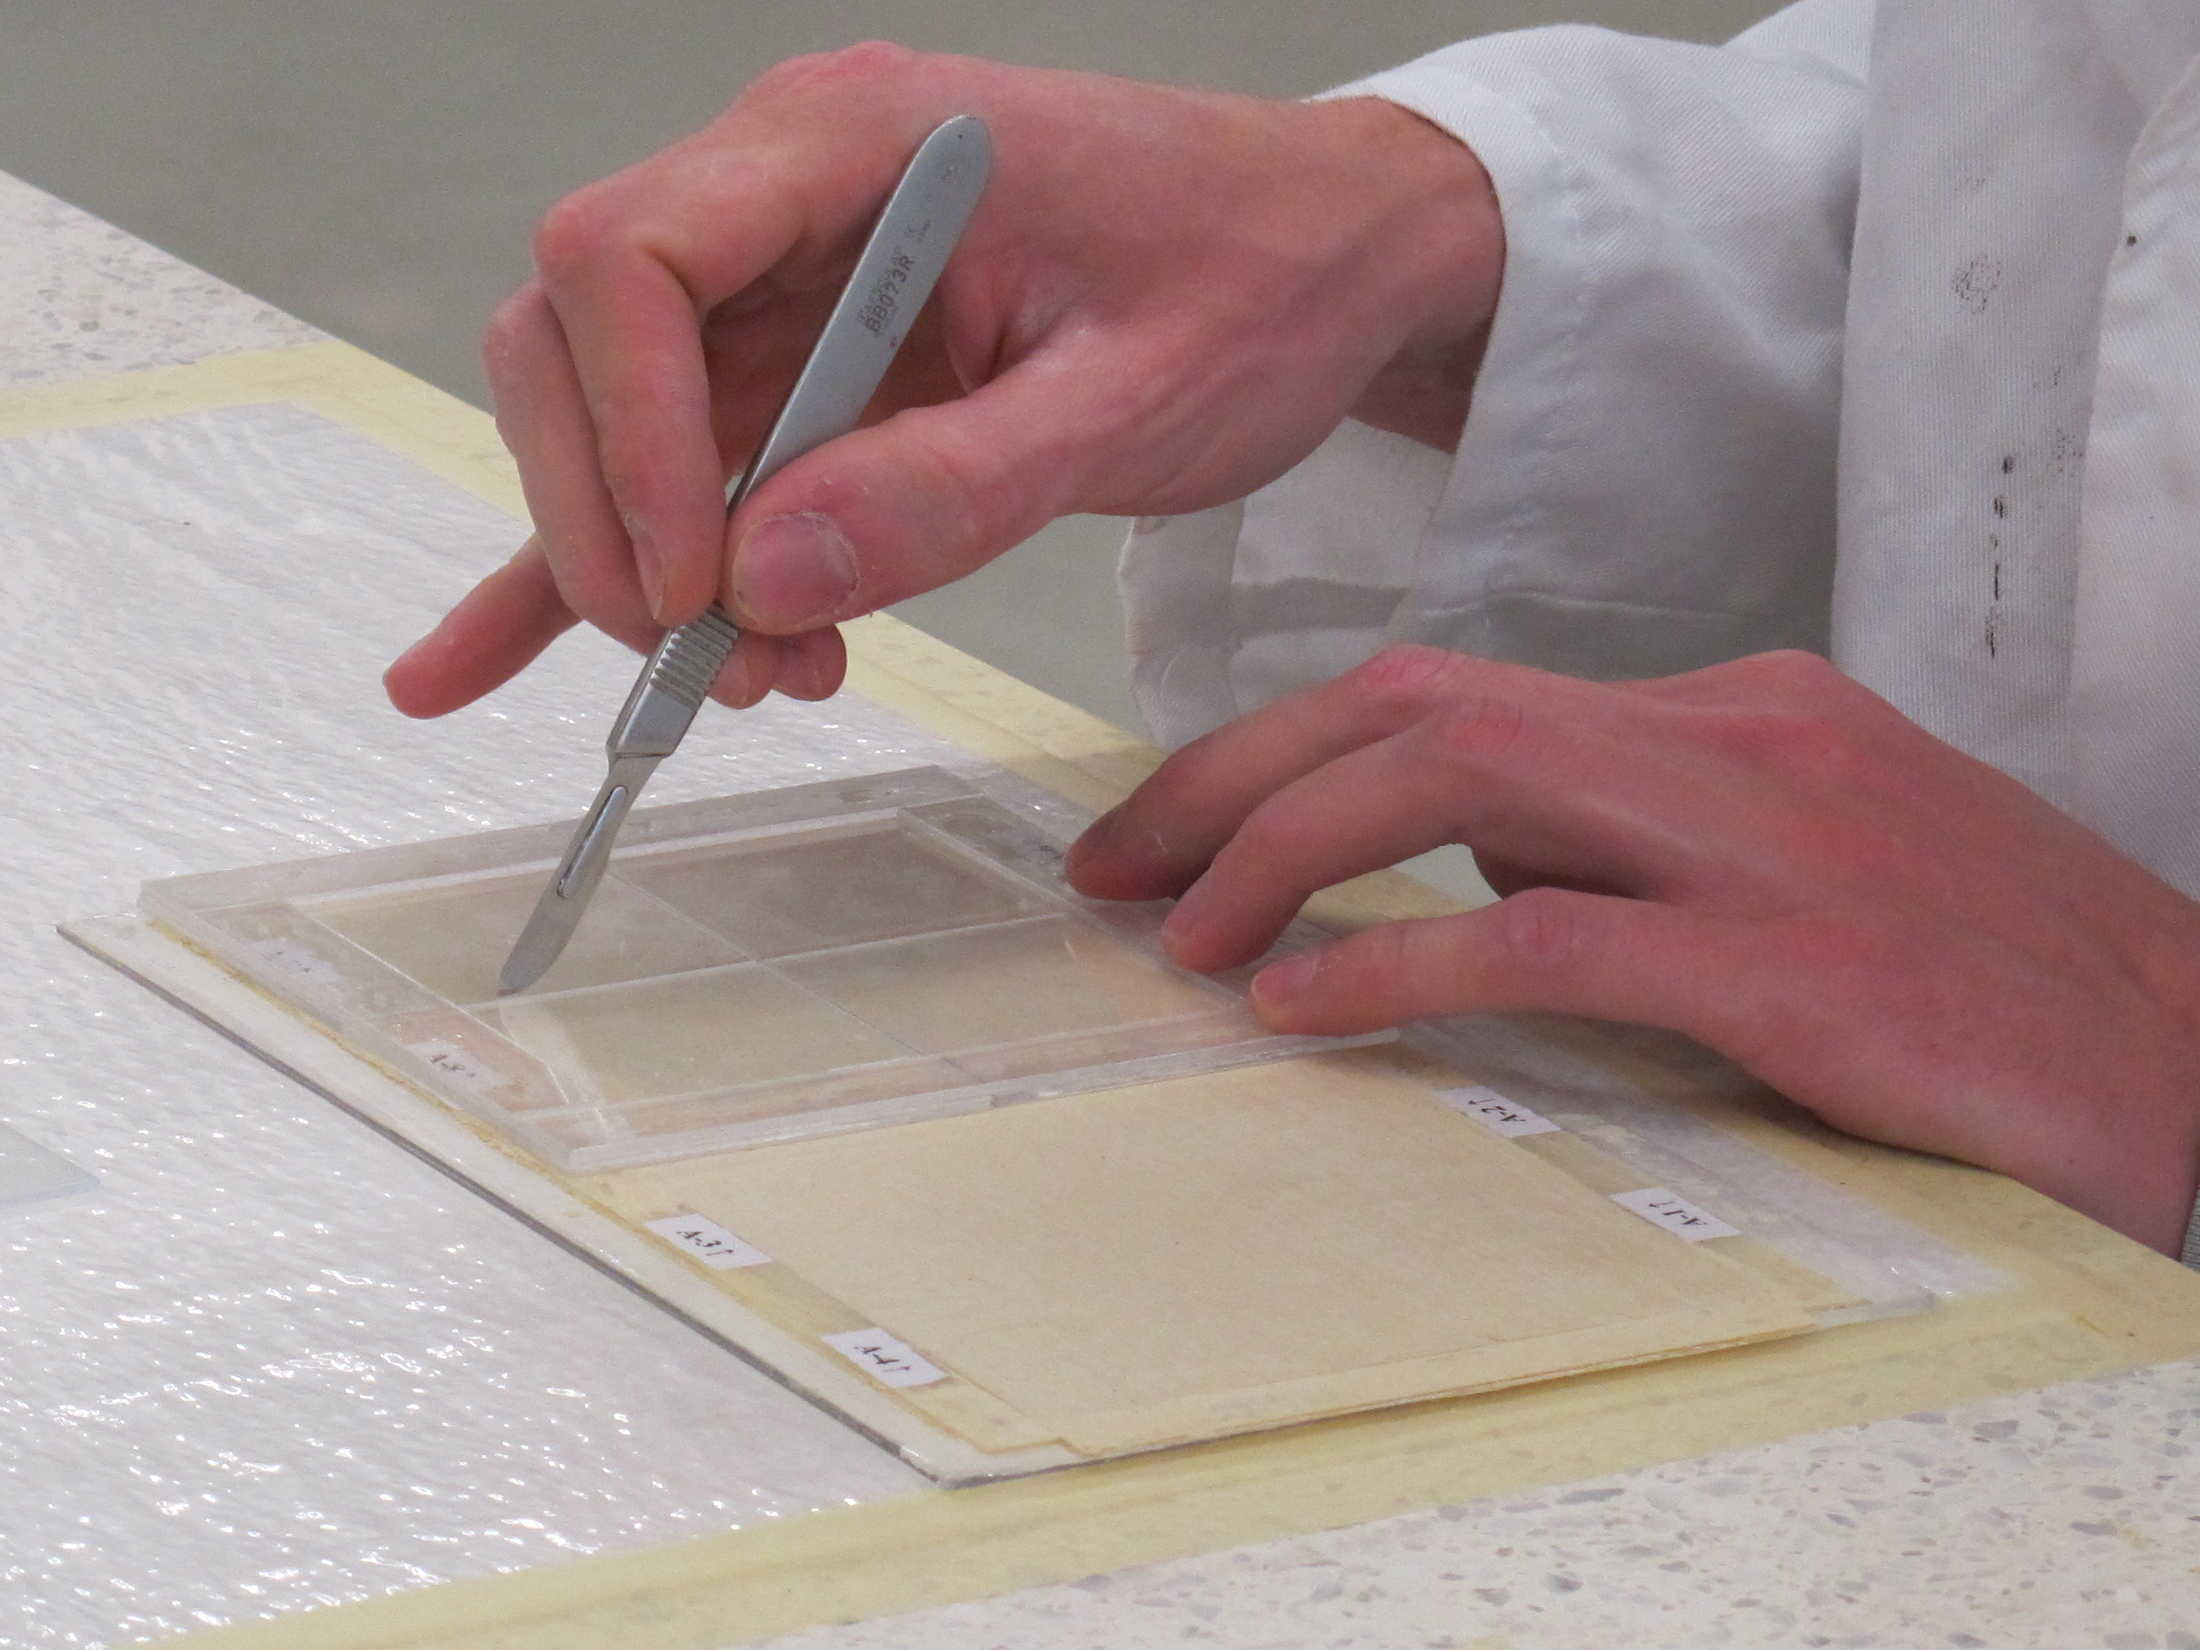
\includegraphics[width=\textwidth]{scoring_01}
    \caption{Scoring of the lime--based paint layer (inner lines)}
    \label{fig:scoring_01}
  \end{minipage}
  \hfill
  \begin{minipage}[t]{0.48\textwidth}
    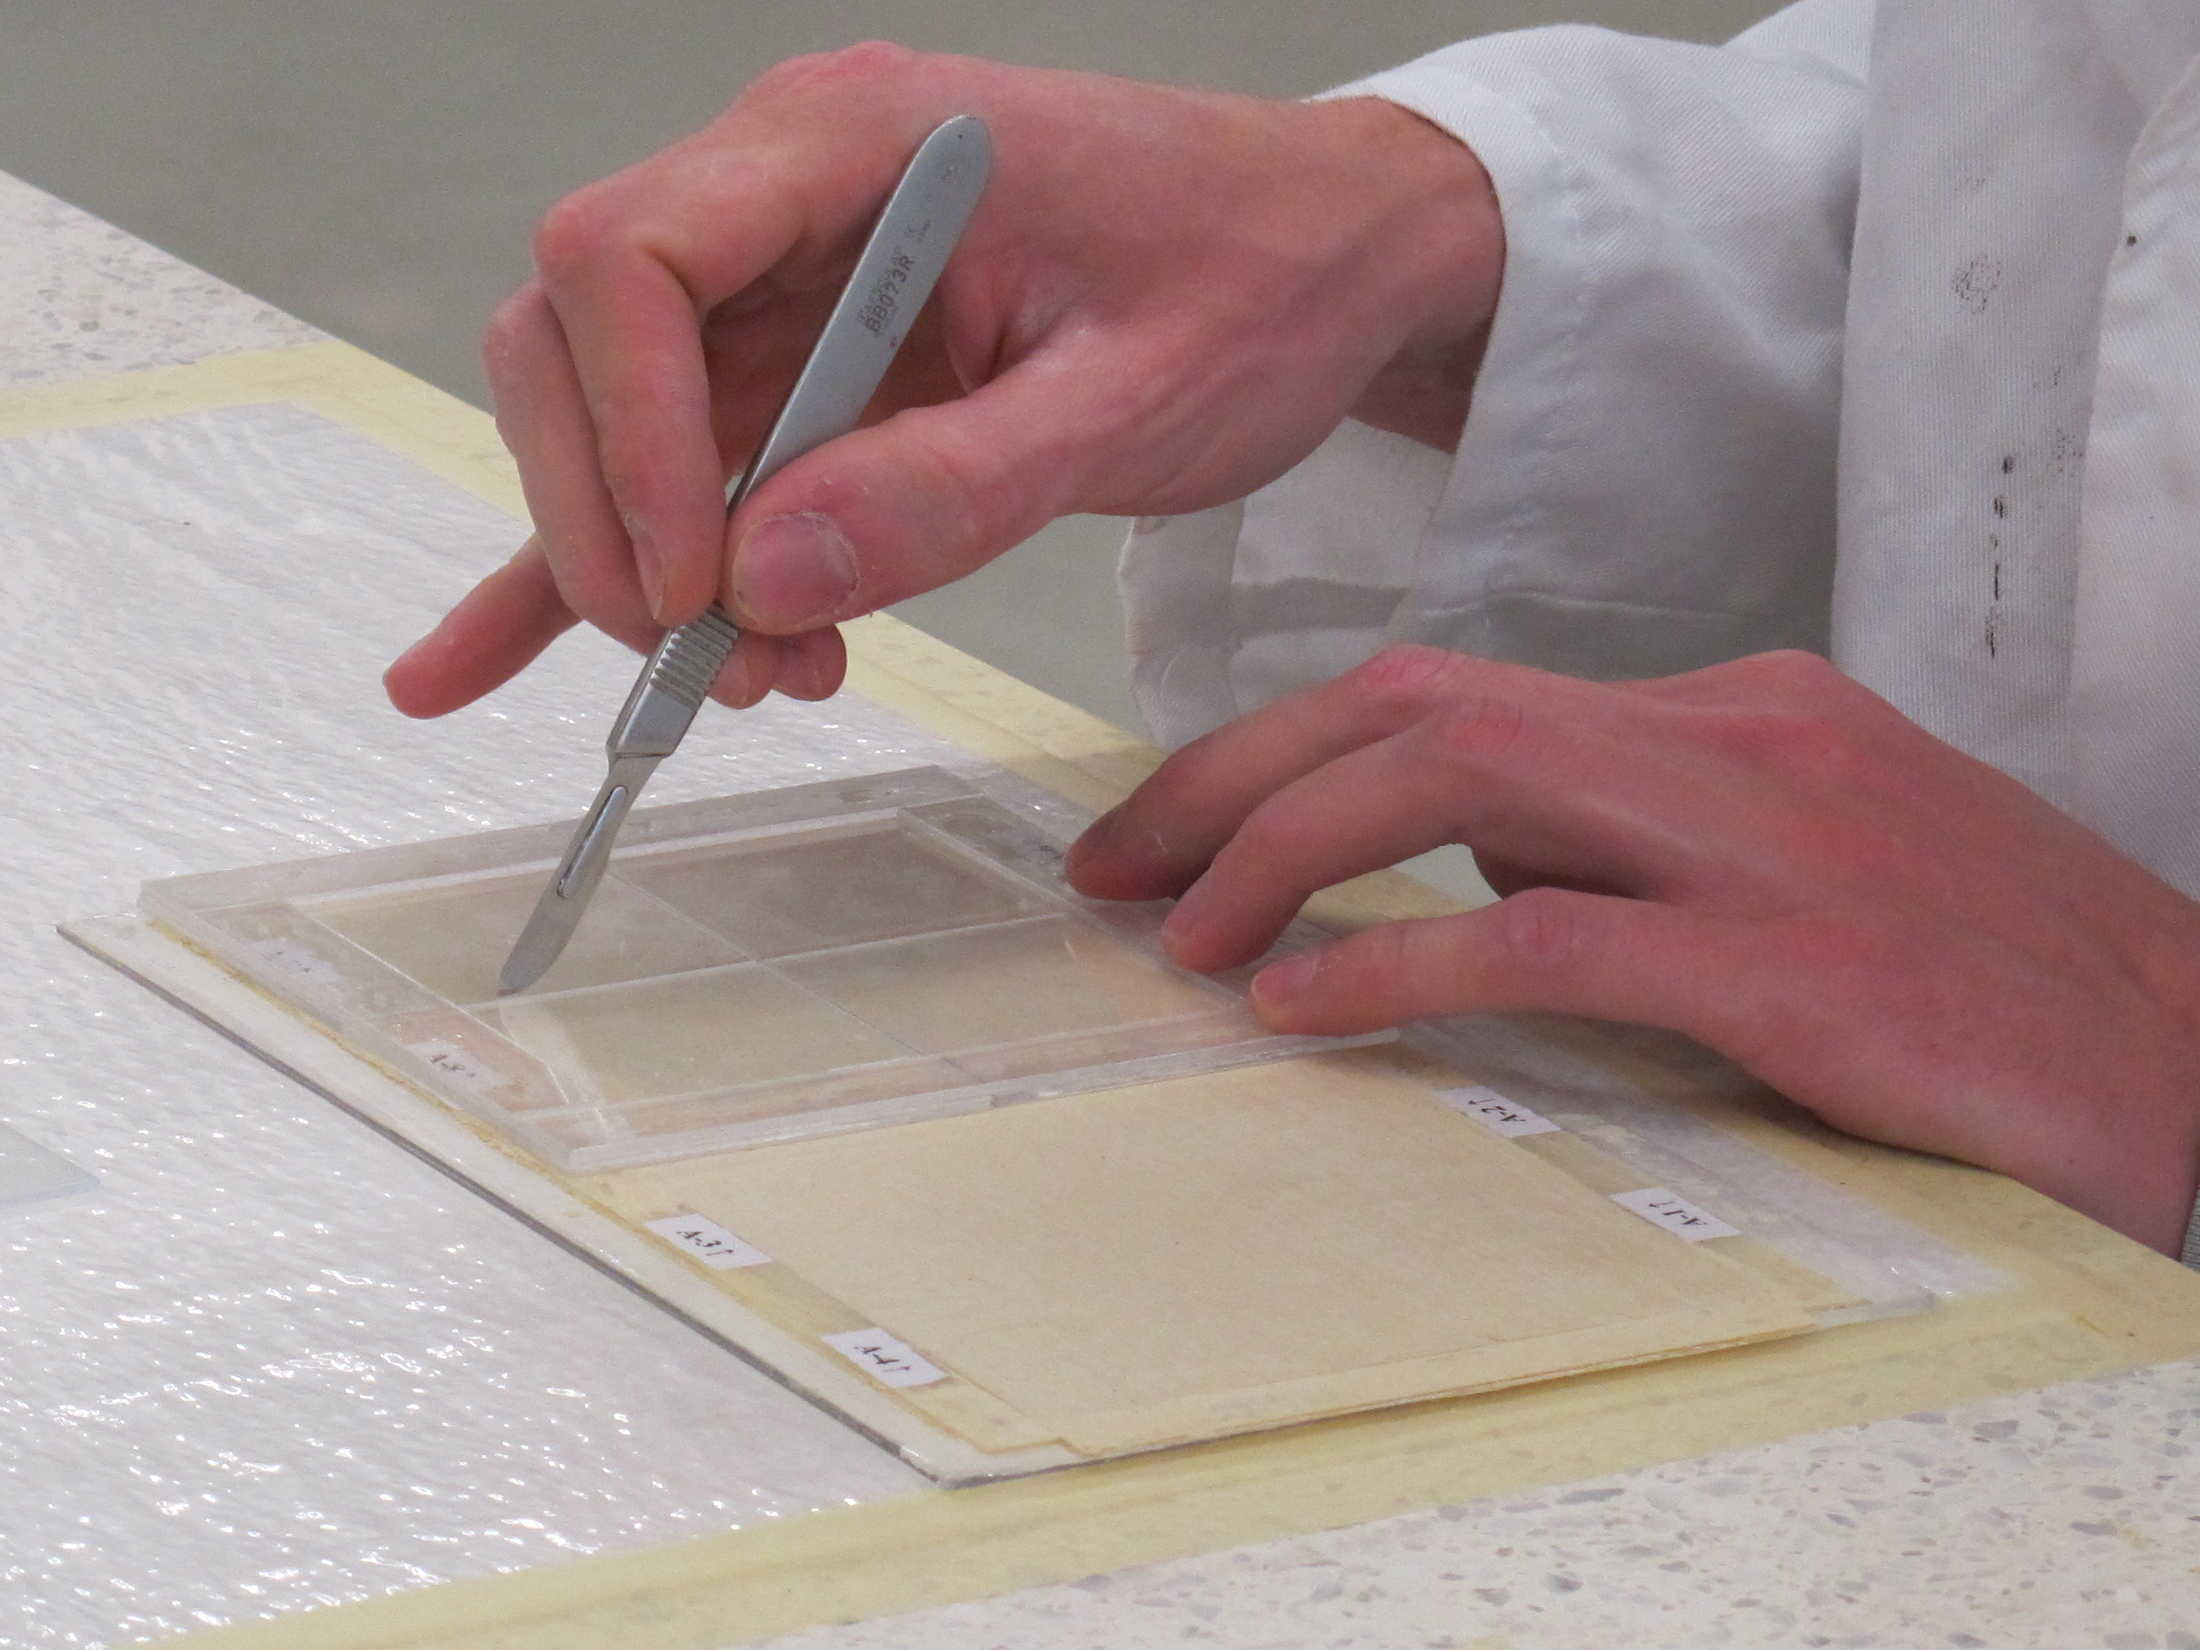
\includegraphics[width=\textwidth]{scoring_01}
    \caption{Scoring of the lime--based paint layer (outline).}
    \label{fig:scoring_02}
  \end{minipage}
\end{figure}

The circumference around the \SI[product-units = single]{9.6 x 9.6}{\cm} square was lightly scored with a scalpel, pressing the \gls{pmma} element onto the surface (Figure~\ref{fig:scoring_02}).
The separation of the different flakes is the most difficult part of the process as the thin and brittle material can be easily damaged.
To accomplish this, the surrounding \ce{CaCO_3}--material was first broken with the scalpel pressing the blade upright on the surface and freeing a \SI[product-units = single]{9.6 x 9.6}{\cm} square.
The blade was then pressed carefully between the individual flakes to separate them.
The individual flakes were not separated until the readhesion intervention.
This helped conserve the integrity of the flakes when moving them was necessary or contact pressure was applied during the colorimetric measurement.

\begin{table}[]
\centering
\caption{tab:description}
\label{Description of the flake imitating layer.}
\begin{tabular}{@{}p{3cm}lp{5cm}@{}}
\toprule
Composition ($Vol$)                                    & Dimensions ($mm$)                                                 & Curing                                                                                          \\ \midrule
\ce{CaCO_3} (2) : yellow ochre (0.1) : slaked lime (1) & \SI[product-units = single]{48 x 48 x 0.5}{} & 1 week RH \SI{95}{\percent}, 3 weeks RH \SI{65}{\percent} with permanent wetting cycles \\
                                                       &                                                      &                                                                                                 \\ \bottomrule
\end{tabular}
\end{table}

\end{document}
